
\chapter{Biztonságos (safe) környezetek}

Ebben a fejezetben bemutatjuk az összes \texttt{safe*} környezetet: \verb|safefigure|, \verb|safetable| és \verb|safemathfigure|.  
Ezek mind tiszteletben tartják a megfelelő logikai kapcsolókat, így szükség esetén egyetlen helyről elrejthetők.  

\section{Külső kép \texttt{safefigure} környezettel}

A külső képfájlokat (például \texttt{.png}, \texttt{.jpg}, \texttt{.pdf}) a \verb|\includegraphics| paranccsal illesztjük be.  
A \verb|safefigure| környezet gondoskodik arról, hogy a \texttt{showfigures} logikai kapcsolóval az összes ábra elrejthető legyen.  

\begin{safefigure}
  \centering
  \includegraphics[width=0.6\textwidth]{img/kittenroar.jpg}
  \caption{Példa külső kép beillesztésére.}
  \label{fig:external-image-example}
\end{safefigure}

\section{Táblázat \texttt{safetable} környezettel}

A táblázatokhoz a \verb|safetable| környezetet használjuk, amely hasonlóan működik, mint a \verb|table|, de tiszteletben tartja a \texttt{showtables} logikai kapcsolót.  

\inputcode[Minta \texttt{safetable} használat]{TeX}{code/ch04-table-example.tex}

\section{Taylor-polinom és Lagrange-maradéktag}

A matematikai képleteket a szokásos \verb|equation| vagy \verb|align| környezettel írjuk.  
Példaként nézzük a Taylor-polinom képletét Lagrange-maradéktaggal.  

Legyen \(f\) \((n+1)\)-szer folytonosan deriválható egy \(a\)-t és \(x\)-et tartalmazó intervallumon.  
Ekkor az \(f\) függvény \(n\)-edfokú Taylor-polinomja az \(a\) pont körül:

\begin{equation}
  T_n(x)
  =
  \sum_{k=0}^{n} \frac{f^{(k)}(a)}{k!} (x-a)^k.
\end{equation}

A függvény értékét az \(n\)-edfokú Taylor-polinom és a maradéktag összegeként írhatjuk:

\begin{equation}
  f(x)
  =
  T_n(x)
  +
  R_{n+1}(x).
\end{equation}

A Lagrange-féle maradéktag alakja:

\begin{equation}
  R_{n+1}(x)
  =
  \frac{f^{(n+1)}(\xi)}{(n+1)!} (x-a)^{n+1},
  \qquad
  \xi \text{ az } a \text{ és } x \text{ közötti pont.}
\end{equation}

Ha ezt grafikonként is ábrázolni szeretnénk, célszerű a \verb|safemathfigure| környezetet használni.  

\section{Irányított gráf \texttt{safemathfigure} és TikZ segítségével}

Az alábbi példa egy három csúcsból álló irányított gráfot mutat, TikZ segítségével, biztonságos matematikai ábraként:  

\begin{safemathfigure}
  \centering
  \begin{tikzpicture}[>=Stealth, node distance=2.5cm]
    \tikzset{vertex/.style={circle,draw,minimum size=1cm}}
    \node[vertex] (v1) {$1$};
    \node[vertex,right=of v1] (v2) {$2$};
    \node[vertex,below=of v1] (v3) {$3$};

    \draw[->] (v1) -- (v2);
    \draw[->] (v2) -- (v3);
    \draw[->] (v1) -- (v3);
  \end{tikzpicture}
  \caption{Egyszerű irányított gráf három csúccsal.}
  \label{fig:directed-graph-example}
\end{safemathfigure}

\section{Függvény grafikonja \texttt{safemathfigure} és \texttt{pgfplots} használatával}

A \texttt{pgfplots} csomaggal függvénygrafikonokat rajzolhatunk közvetlenül a \LaTeX{} dokumentumban.  
Az alábbi példa a \(y = \sin x\) függvényt ábrázolja az \([0, 2\pi]\) intervallumon:  

\begin{safemathfigure}
  \centering
  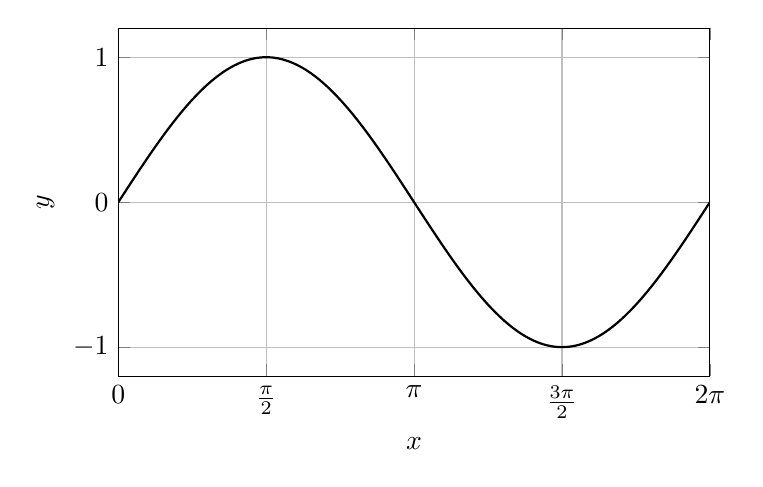
\begin{tikzpicture}
    \begin{axis}[
      width=0.75\textwidth,
      height=6cm,
      xlabel={$x$},
      ylabel={$y$},
      domain=0:6.28318,
      samples=200,
      grid=both,
      xmin=0, xmax=6.28318,
      ymin=-1.2, ymax=1.2,
      xtick={0,1.5708,3.1416,4.7124,6.2832},
      xticklabels={$0$, $\frac{\pi}{2}$, $\pi$, $\frac{3\pi}{2}$, $2\pi$},
    ]
      \addplot[thick] {sin(deg(x))};
    \end{axis}
  \end{tikzpicture}
  \caption{$y = \sin x$ grafikonja az $[0, 2\pi]$ intervallumon.}
  \label{fig:sin-plot-example}
\end{safemathfigure}
\newpage
\section{Matematikai ábrák kikapcsolása}

Ha a dolgozat egy vázlatosabb verzióját szeretnénk generálni, előfordulhat, hogy a matematikai ábrákat ideiglenesen el szeretnénk rejteni.  
Ezt megtehetjük a \texttt{showmathfigures} logikai kapcsolóval, amely a \texttt{szte-thesis.cls} fájlban van definiálva.  

\begin{codeblock}[caption={Matematikai ábrák kikapcsolása}]{TeX}
\setboolean{showmathfigures}{false}
\end{codeblock}

\section{UML diagramok (kikapcsolható ábrák)}

Ebben a részben néhány gyakori UML diagramtípust mutatunk be.
Minden példa \texttt{safefigure} környezetben van.
A példák forrása a \texttt{code/} mappában található.
A fejezetben az \verb|\inputcode| parancs importálja a forrást.
A PDF-ben az ábra a \verb|\input{...}| paranccsal kerül be.

\subsection{UML osztálydiagram (class diagram)}

\inputcode[UML class diagram forras]{TeX}{code/ch04-uml-class.tex}

\begin{safefigure}
	\centering
	\begin{tikzpicture}
  \umlclass[x=0,y=0]{User}
  {+id: int\\+name: string}
  {+login()\\+logout()}

  \umlclass[x=6,y=0]{Order}
  {+number: string\\+createdAt: date}
  {+total(): money}

  \umlclass[x=3,y=-3]{OrderItem}
  {+sku: string\\+qty: int}
  {}

  \umluniassoc[mult1=1,mult2=0..*]{User}{Order}
  \umlcompo[mult2=1..*]{Order}{OrderItem}
\end{tikzpicture}


	\caption{UML osztalydiagram pelda.}
	\label{fig:uml-class}
\end{safefigure}

\subsection{UML szekvenciadiagram (sequence diagram)}

\inputcode[UML sequence diagram forras]{TeX}{code/ch04-uml-sequence.tex}

\begin{safefigure}
	\centering
	\begin{sequencediagram}
  \newthread{u}{User}
  \newinst{c}{Controller}
  \newinst{s}{Service}
  \newinst{r}{Repo}

  \begin{call}{u}{createOrder()}{c}{orderId}
    \begin{call}{c}{validate()}{s}{ok}
    \end{call}
    \begin{call}{c}{save(order)}{r}{ok}
    \end{call}
  \end{call}
\end{sequencediagram}


	\caption{UML szekvenciadiagram pelda.}
	\label{fig:uml-sequence}
\end{safefigure}

\subsection{UML use case diagram}

\inputcode[UML use case diagram forras]{TeX}{code/ch04-uml-usecase.tex}

\begin{safefigure}
	\centering
	\begin{tikzpicture}
	\umlactor[x=0,y=0]{User}
	
	\begin{umlsystem}[x=5,y=0]{WebApp}
		\umlusecase[name=ucLogin,y=1]{Login}
		\umlusecase[name=ucPlaceOrder,y=-1]{PlaceOrder}
		\umlusecase[name=ucTrackOrder,y=-3]{TrackOrder}
	\end{umlsystem}
	
	\umlassoc{User}{ucLogin}
	\umlassoc{User}{ucPlaceOrder}
	\umlassoc{User}{ucTrackOrder}
\end{tikzpicture}

	\caption{UML use case diagram pelda.}
	\label{fig:uml-usecase}
\end{safefigure}

\subsection{Allapotgep diagram (state machine jellegu)}

\inputcode[Allapotgep diagram forras]{TeX}{code/ch04-uml-state.tex}

\begin{safefigure}
	\centering
	\begin{tikzpicture}[>=Stealth, node distance=3.2cm, on grid, auto]
  \node[state, initial] (new) {NEW};
  \node[state, right=of new] (paid) {PAID};
  \node[state, below=of paid] (shipped) {SHIPPED};
  \node[state, right=of shipped] (done) {DONE};
  \node[state, below=of new] (canceled) {CANCELED};

  \path[->]
    (new) edge node {pay} (paid)
    (paid) edge node {ship} (shipped)
    (shipped) edge node {deliver} (done)
    (new) edge node {cancel} (canceled)
    (paid) edge node {cancel} (canceled);
\end{tikzpicture}


	\caption{Allapotgep pelda (UML state machine jelleg).}
	\label{fig:uml-state}
\end{safefigure}

